\let\negmedspace\undefined
\let\negthickspace\undefined
\documentclass[journal]{IEEEtran}
\usepackage[a5paper, margin=10mm, onecolumn]{geometry}
%\usepackage{lmodern} % Ensure lmodern is loaded for pdflatex
\usepackage{tfrupee} % Include tfrupee package

\setlength{\headheight}{1cm} % Set the height of the header box
\setlength{\headsep}{0mm}     % Set the distance between the header box and the top of the text

\usepackage{gvv-book}
\usepackage{gvv}
\usepackage{cite}
\usepackage{amsmath,amssymb,amsfonts,amsthm}
\usepackage{algorithmic}
\usepackage{graphicx}
\usepackage{textcomp}
\usepackage{xcolor}
\usepackage{txfonts}
\usepackage{listings}
\usepackage{enumitem}
\usepackage{mathtools}
\usepackage{gensymb}
\usepackage{comment}
\usepackage[breaklinks=true]{hyperref}
\usepackage{tkz-euclide} 
\usepackage{listings}
% \usepackage{gvv}                                        
\def\inputGnumericTable{}                                 
\usepackage[latin1]{inputenc}                                
\usepackage{color}                                            
\usepackage{array}                                            
\usepackage{longtable}                                       
\usepackage{calc}                                             
\usepackage{multirow}                                         
\usepackage{hhline}                                           
\usepackage{ifthen}                                           
\usepackage{lscape}
\begin{document}

\bibliographystyle{IEEEtran}
\vspace{3cm}

\title{1.8.28}
\author{EE25BTECH11011 - Navya}
% \maketitle
% \newpage
% \bigskip
{\let\newpage\relax\maketitle}

\renewcommand{\thefigure}{\theenumi}
\renewcommand{\thetable}{\theenumi}
\setlength{\intextsep}{10pt} % Space between text and floats

\textbf{Question}:\\
Find the equation of the set of the points $P$ such that its distances 
from the points $A(3,4,-5)$ and $B(-2,1,4)$ are equal.\\

\textbf{Solution:} \\

Let the required point be denoted by the vector $\Vec{X}\in\mathbb{R}^3$.  
The condition that $\Vec{X}$ is equidistant from $\Vec{A}$ and $\Vec{B}$ can be written using the norm (distance) as
\begin{align}
\lVert \Vec{X} - \Vec{A} \rVert = \lVert \Vec{X} - \Vec{B} \rVert.
\end{align}

Squaring both sides (to remove the square root) gives
\begin{align}
\lVert \Vec{X} - \Vec{A} \rVert^2 = \lVert \Vec{X} - \Vec{B} \rVert^2.
\end{align}

Using $\lVert \Vec{u}\rVert^2 = \Vec{u}^T\Vec{u}$, expand both sides:
\begin{align}
(\Vec{X}-\Vec{A})^T(\Vec{X}-\Vec{A}) &= (\Vec{X}-\Vec{B})^T(\Vec{X}-\Vec{B}).
\end{align}

Expanding the products yields
\begin{align}
\Vec{X}^T\Vec{X} - 2\Vec{A}^T\Vec{X} + \Vec{A}^T\Vec{A}
&= \Vec{X}^T\Vec{X} - 2\Vec{B}^T\Vec{X} + \Vec{B}^T\Vec{B}.
\end{align}

The $\Vec{X}^T\Vec{X}$ terms cancel, leaving a linear equation in $\Vec{X}$:
\begin{align}
-2\Vec{A}^T\Vec{X} + \Vec{A}^T\Vec{A} &= -2\Vec{B}^T\Vec{X} + \Vec{B}^T\Vec{B}.
\end{align}

Rearrange to isolate the inner product with $\Vec{X}$:
\begin{align}
2(\Vec{B}-\Vec{A})^T \Vec{X} &= \Vec{B}^T\Vec{B} - \Vec{A}^T\Vec{A}.
\end{align}

Now compute the two vector/scalar pieces on the right:

\begin{align}
\Vec{B}-\Vec{A} &= \myvec{-2\\1\\4} - \myvec{3\\4\\-5} = \myvec{-5\\-3\\9}, \\[6pt]
\Vec{B}^T\Vec{B} &= (-2)^2 + 1^2 + 4^2 = 21, \\[2pt]
\Vec{A}^T\Vec{A} &= 3^2 + 4^2 + (-5)^2 = 50.
\end{align}

Substitute these values into the linear equation:
\begin{align}
2\myvec{-5 & -3 & 9}\,\Vec{X} &= 21 - 50 = -29.
\end{align}

Simplify the left-hand side:
\begin{align}
\myvec{-10 & -6 & 18}\,\Vec{X} &= -29.
\end{align}

Hence the equation of the plane is given by:
$\boxed{\;\myvec{-10 & -6 & 18}\,\Vec{X} = -29\;}$

\begin{figure}[h]
    \centering
    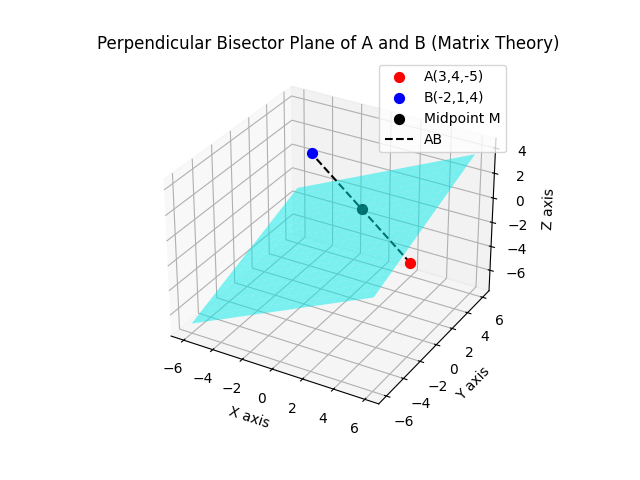
\includegraphics[height=0.5\textheight, keepaspectratio]{figs/fig2.png}
    \label{figure_1}
\end{figure}

\end{document}

